\documentclass[polish,12pt]{aghthesis}
% \documentclass[english,12pt]{aghthesis} dla pracy w jêzyku angielskim. Uwaga, w przypadku strony tytu³owej zmiana jêzyka dotyczy tylko kolejno¶ci wersji jêzykowych tytu³u pracy. 

% Szablon przystosowany jest do druku dwustronnego. 

\usepackage[T1]{fontenc}
\usepackage[utf8]{inputenc}
\usepackage{url}

\author{Mateusz Bielesz, Wojciech Kosior, Marek Moryl, Kamil Szarek}

\titleProject{Weryfikacja poprawności wyników zwracanych przez serwery DNS \linebreak dla serwisu klienta}

\titleDocument{Podsumowanie pierwszego i zakres drugiego sprintu}

\fieldofstudy{Informatyka}

\supervisor{mgr\ inż.\ Witold Rakoczy}


\date{\the\year}


\begin{document}

\maketitle

\section{Zadania zrealizowane}

\subsection*{Front-end}
\begin{itemize}
  \item zrealizowana strona główna, dostępna dla użytkowników niezalogowanych,
  \item rozbudowany moduł administratora, zapewniający pełną obsługę użytkowników,
  \item zrealizowana strona rejestracji nowego użytkownika,
  \item strona rejestracji jest w pełni funkcjonalna, sprawdza wprowadzone wartości, jeśli są poprawne dodaje nowego użytkownika do bazy danych, 
  \item zrealizowana strona logowania,
  \item strona logowania zapewnia autentykację użytkownika, po wprowadzeniu błędnych danych wypisuje komunikat "Username or password is incorrect", po wprowadzeniu poprawnych danych przekierowuje do strony głównej, 
\end{itemize}

\subsection*{Back-end}
\begin{itemize}
  \item Tworzenie namespacu i uruchomianie procesu w namespace'ie 
  \item Obsługa openVPN z poziomu konsoli 
  \item Przekierowanie na interfejs openVPN ruchu z namespac'u 
  \item Obsługa zapytań do bazy danych z poziomu pythona
  \item Projekt struktury bazy danych
\end{itemize}

\newpage

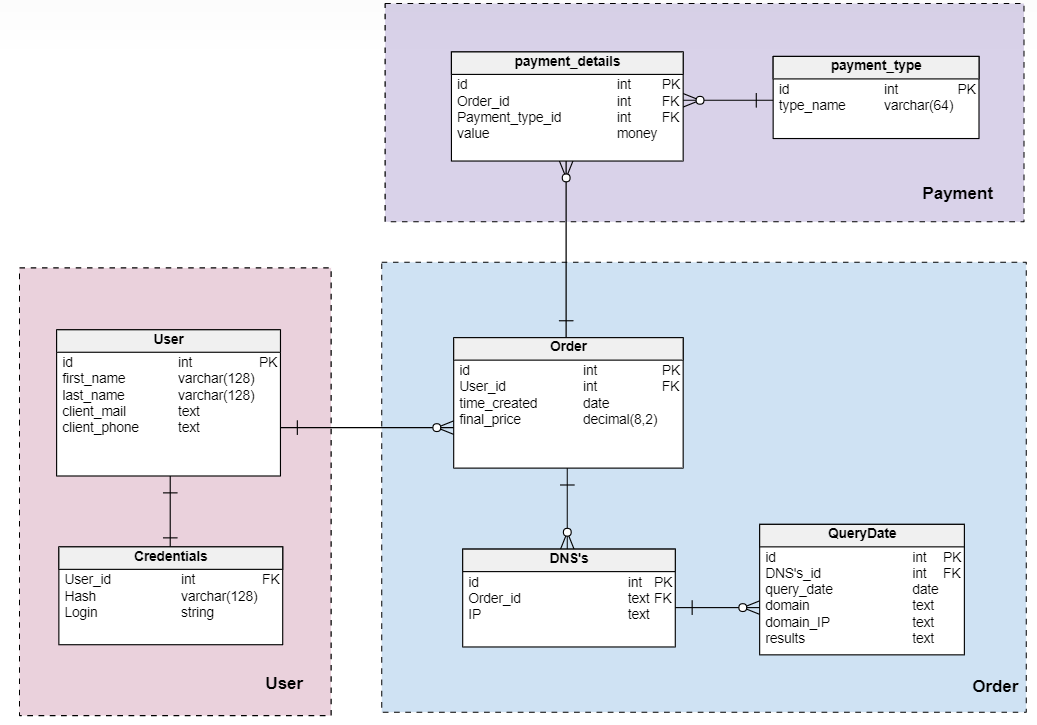
\includegraphics[scale=0.6]{db_schema.png}


\newpage

\section{Backlog projektu}

\subsection*{Front-end}
\begin{itemize}
  \item stworzenie strony użytkownika, do której zostanie on przekierowany po zalogowaniu,
  \item udostępnienie użytkownikowi możliwości wprowadzenia danych serwisu, który ma być obsługiwany przez backend,
  \item utworzenie formularza informującego o niepoprawnym działaniu serwera DNS, 
  \item udostępnienie użytkownikowi danych o serwisach które wprowadził do systemu,
  \item udostępnienie użytkownikowi możliwości anulowania subskrypcji,
  \item udostępnienie użytkownikowi statystyk dotyczących jego serwisów,
  \item obrazowanie statystyk w ładnej formie graficznej,
  \item dodanie podstron strony głównej, dotyczących opisu projektu, działania systemu,
\end{itemize}

\subsection*{Back-end}
\begin{itemize}
    \item Umieszczenie bazy danych na zewnętrznym serwerze 
    \item Robienie zapisów i odczytów z bazy danych 
    \item Scalenie poszczególnych funkcjonalności 
\end{itemize}

\newpage

\section{Zadania do zrealizowania w drugim sprincie}

\subsection*{Front-end}
\begin{itemize}
  \item zmiana bazy danych na PostgreSQL, kompatybilną z back-endem,
  \item budowa podstawowej strony użytkownika, do której zostałby przekierowany po zalogowaniu i miałby możliwość wykupienia naszej usługi,
\end{itemize}
\begin{list}{$\circ$}{} 
  \item stworzenie loga produktu,
  \item uzupełnienie podstron strony głównej opisami.
\end{list}

\subsection*{Back-end}
\begin{itemize}
    \item Umieszczenie bazy danych na zewnętrznym serwerze 
    \item Robienie zapisów i odczytów z bazy danych 
\end{itemize}
\end{document}
